A Figura~\ref{fig:hiper} apresenta a mediana de 51 rodadas de resposta do algortimo xNES a variações tanto do
tamanho da população, quanto da taxa de aprendizado $\eta_A$.
Diferentemente da matriz $A$ que pertence ao $\mathbb{R}^{d \times d}$, o valor $\mu$ pertence ao $\mathbb{R}^{d}$, sendo
mais fácil de ser encontrado adaptativamente.
Portanto, o parâmetro $\eta_{\mu}$ não foi mantido com valor recomendado.

A partir da Figura~\ref{fig:hiper}, pode-se fazer algumas considerações.
Percebe-se que para baixos valores de $\eta_A$, como $0,0033$, o algoritmo tem seu pior desempenho em todas as funções
de avaliação, com exceção da Função 14.
Esse pode ser um indicativo que para este valor de taxa de aprendizado o algoritmo necessite de mais avaliações para
obter sucesso.

Para populações com maior número de indivíduos, maiores taxas de aprendizado costumam ser melhores mas novamente a Função 14
não apresenta esse comportamento.
Uma possível explicação para esse fenômeno é encontrada na maior pressão nos indíduos devido ao tamanho da população, sendo
assim o algoritmo beneficiado pela maior capacidade exploratória provinda de altas taxas de aprendizado.

Outra observação a ser feita em relação ao tamanho da população: utilizando-se menos indivíduos, $8$ ou $13$, taxas de
aprendizado baixas ou altas demais resultam em pior performance quando comparadas a utilização de valores como $0,02$ ou
$0.033$.

Conclui-se que, dada a variedade de funções objetivo e as diferentes dimensionalidades, não se pode apontar um vencedor absoluto.
Funções distintas se sobressaem com diferentes parâmetros.
Entretanto, notou-se que a combinação de parâmetros que melhor generalizou foi a de tamanho $21$ de população e taxa de
aprendizado $\eta_A = 0,033$.

\begin{figure*}[!t]
\centering
\subfloat{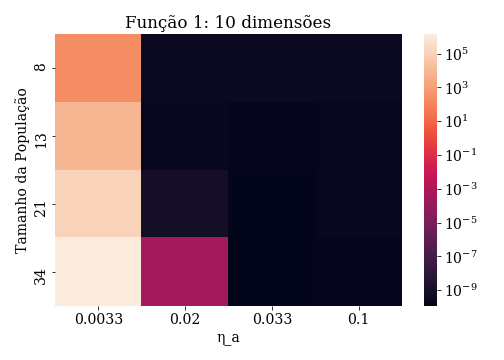
\includegraphics[width=2.0in]{figures/hiper_selection/function=01_dim=10.png}
\label{fig:func01dim10}}
\subfloat{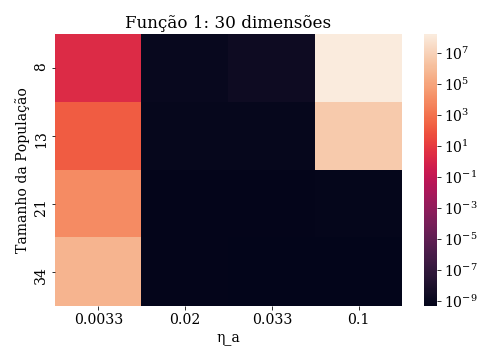
\includegraphics[width=2.0in]{figures/hiper_selection/function=01_dim=30.png}
\label{fig:func01dim30}}
\hfil
\subfloat{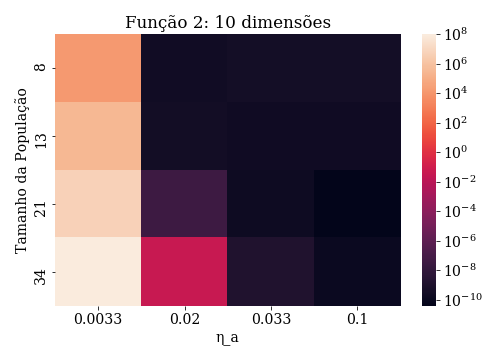
\includegraphics[width=2.0in]{figures/hiper_selection/function=02_dim=10.png}
\label{fig:func02dim10}}
\subfloat{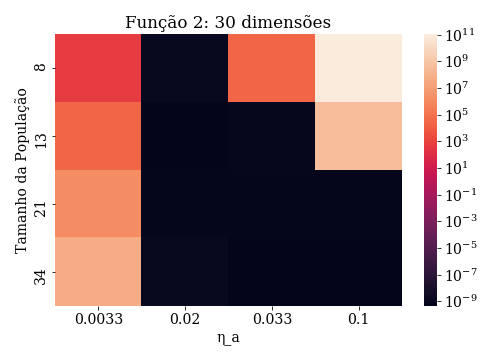
\includegraphics[width=2.0in]{figures/hiper_selection/function=02_dim=30.png}
\label{fig:func02dim30}}
\hfil
\subfloat{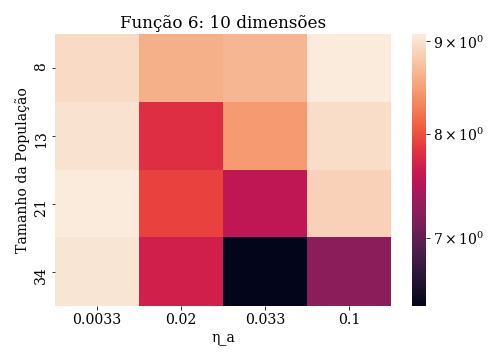
\includegraphics[width=2.0in]{figures/hiper_selection/function=06_dim=10.png}
\label{fig:func06dim10}}
\subfloat{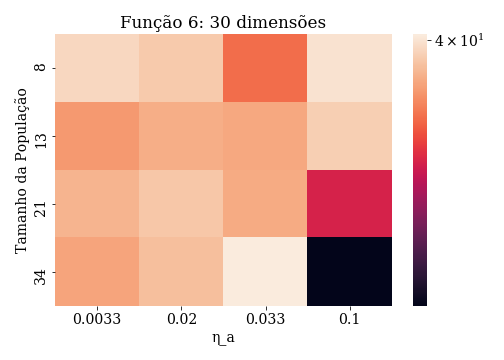
\includegraphics[width=2.0in]{figures/hiper_selection/function=06_dim=30.png}
\label{fig:func06dim30}}
\hfil
\subfloat{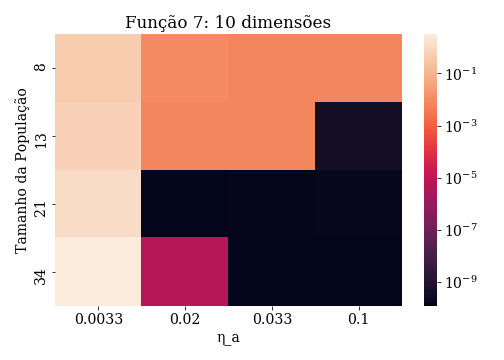
\includegraphics[width=2.0in]{figures/hiper_selection/function=07_dim=10.png}
\label{fig:func07dim10}}
\subfloat{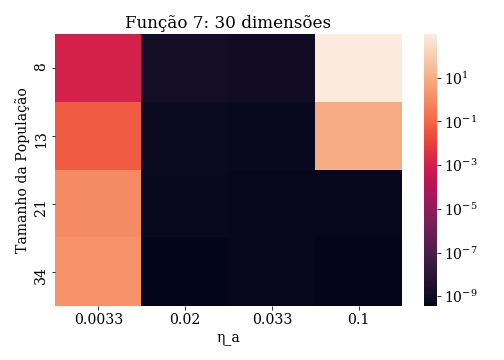
\includegraphics[width=2.0in]{figures/hiper_selection/function=07_dim=30.png}
\label{fig:func07dim30}}
\hfil
\subfloat{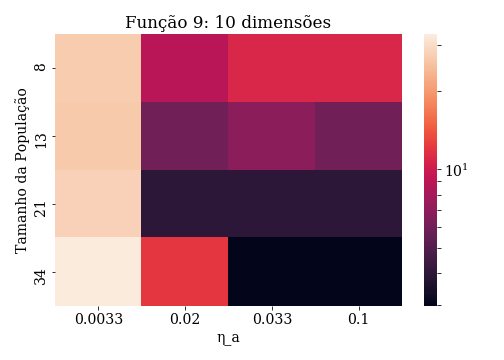
\includegraphics[width=2.0in]{figures/hiper_selection/function=09_dim=10.png}
\label{fig:func09dim10}}
\subfloat{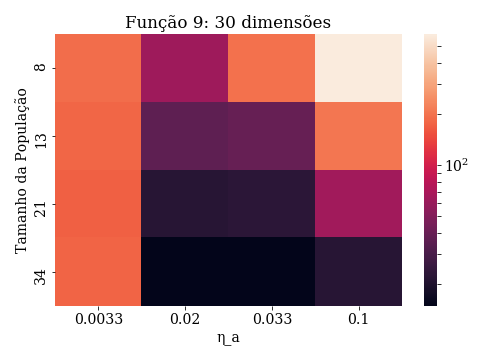
\includegraphics[width=2.0in]{figures/hiper_selection/function=09_dim=30.png}
\label{fig:func09dim30}}
\hfil
\subfloat{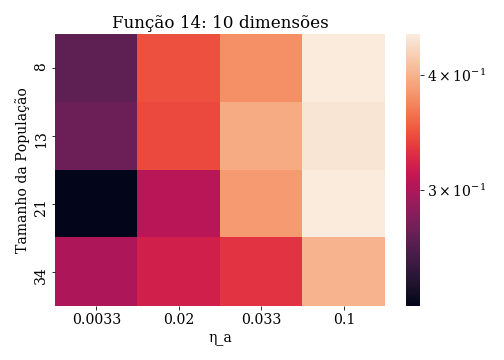
\includegraphics[width=2.0in]{figures/hiper_selection/function=14_dim=10.png}
\label{fig:func14dim10}}
\subfloat{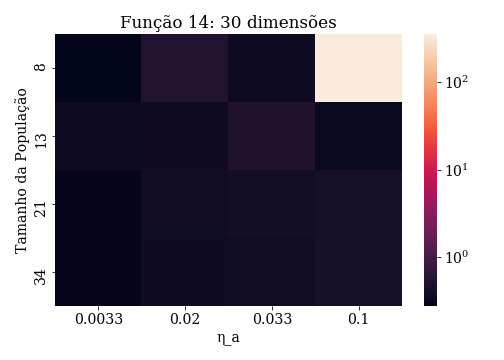
\includegraphics[width=2.0in]{figures/hiper_selection/function=14_dim=30.png}
\label{fig:func14dim30}}
\caption{Seleção de hiperparâmetros do xNES}
\label{fig:hiper}
\end{figure*}

Seguindo para a fase de comparação entre os algoritmos, a Figura~\ref{fig:comp} apresenta o erro de aptidão obtido por
cada algoritmo.
Nessa figura comparamos o xNES com os parâmetros selecionados na fase anterior, o xNES com seus valores originalmente
apresentados pelos autores e o CMA-ES também com seus valores padrão.
Assim como na etapa anterior, cada algoritmo foi rodado 51 vezes para cada função.

A primeira consideração a se feita é que para as funções $1$ e $2$ todos algoritmos foram capazes de obter sucesso, ou seja,
erro menor que $10^{-8}$, dentro do número permitido de avaliações da função objetivo.
Observamos ainda nas funções $1$ e $2$ que o algoritmo xNES com parâmetros pré-selecionados apresentou menor média e
variância de aptidão.

Analisando a função $6$, ressalta-se que o algoritmo CMA-ES foi o único a conseguir obter sucesso no problema com $10$
dimensões, porém em apenas uma das 51 rodadas.
Considerando ainda as $10$ dimensões, o CMA-ES superou o xNES com valores originais porém esta dentro da margem de
erro do xNES com parâmetros selecionados apesar de apresentar melhor média.
Por sua vez, para função $7$ com $30$ dimensões o CMA-ES superou os outros dois algoritmos que apresentaram resultados
iguais entre si.

A função $7$ apresenta um comportamento atípico, os resultados em $30$ dimensões para todos algoritmos foram superiores
aos resulados de $10$ dimensões.
Nesta função a variação de parâmetros do xNES se mostrou irrelevante.
Analisando o problema com 10 dimensões, o CMA-ES apresentou a maior média de erro e obteve sucesso apenas em 25\% das
rodadas enquanto os xNES obtiveram 50\% de sucesso, porém, os resultados ainda se encontram dentro da barra de erro.
Avaliando o problema com $30$ dimensões os xNES obtiveram sucesso em todos os casos enquanto o CMA-ES atingiu 84\%.

As funções $9$ e $14$ apresentam resultados parecidos.
Nestas avaliações os algoritmos apresentaram poucas diferenças entre si e com resultados dentro da margens de erros.

\begin{figure*}[!t]
\centering
\subfloat{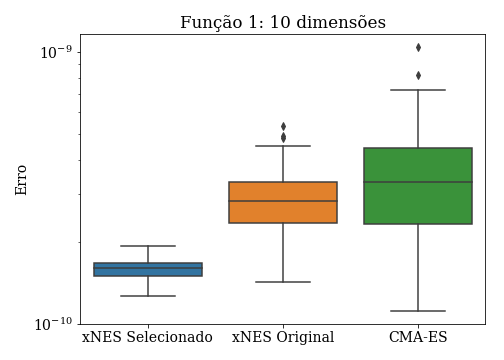
\includegraphics[width=2.0in]{figures/analysis_results/function=01_dim=10.png}
\label{fig:result_func01dim10}}
\subfloat{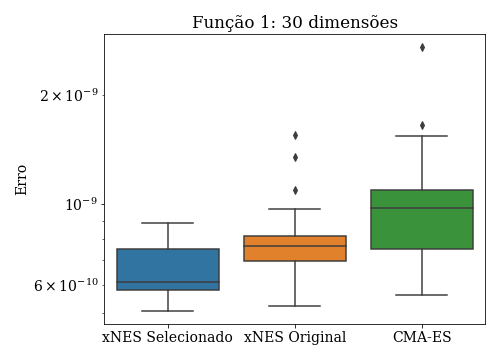
\includegraphics[width=2.0in]{figures/analysis_results/function=01_dim=30.png}
\label{fig:result_func01dim30}}
\hfil
\subfloat{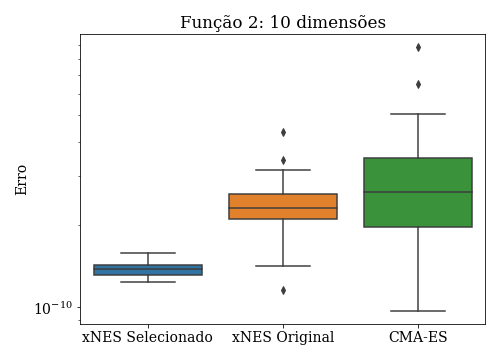
\includegraphics[width=2.0in]{figures/analysis_results/function=02_dim=10.png}
\label{fig:result_func02dim10}}
\subfloat{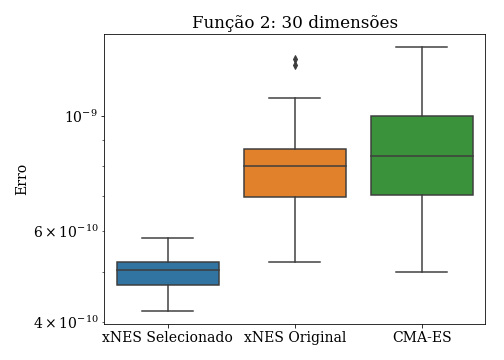
\includegraphics[width=2.0in]{figures/analysis_results/function=02_dim=30.png}
\label{fig:result_func02dim30}}
\hfil
\subfloat{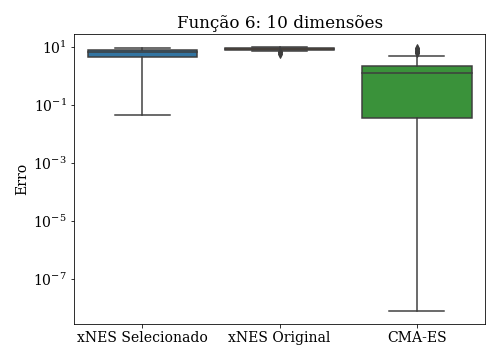
\includegraphics[width=2.0in]{figures/analysis_results/function=06_dim=10.png}
\label{fig:result_func06dim10}}
\subfloat{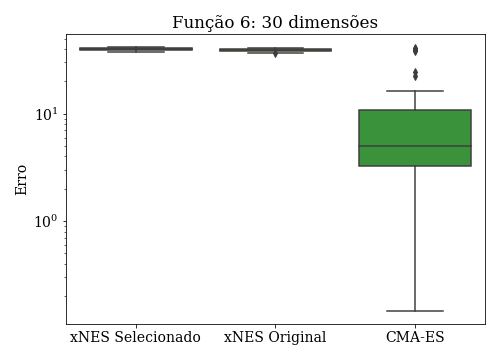
\includegraphics[width=2.0in]{figures/analysis_results/function=06_dim=30.png}
\label{fig:result_func06dim30}}
\hfil
\subfloat{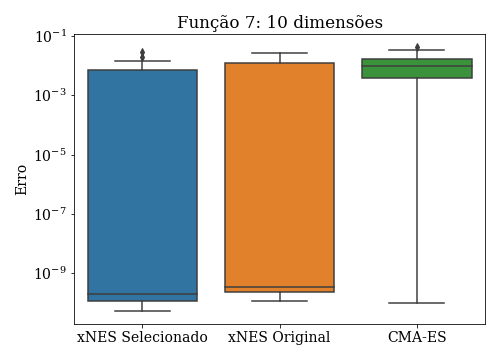
\includegraphics[width=2.0in]{figures/analysis_results/function=07_dim=10.png}
\label{fig:result_func07dim10}}
\subfloat{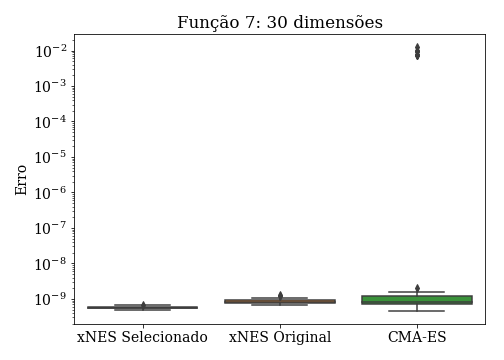
\includegraphics[width=2.0in]{figures/analysis_results/function=07_dim=30.png}
\label{fig:result_func07dim30}}
\hfil
\subfloat{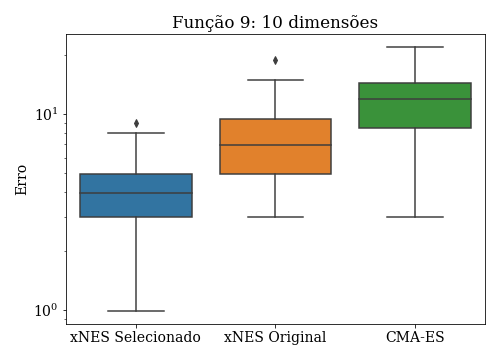
\includegraphics[width=2.0in]{figures/analysis_results/function=09_dim=10.png}
\label{fig:result_func09dim10}}
\subfloat{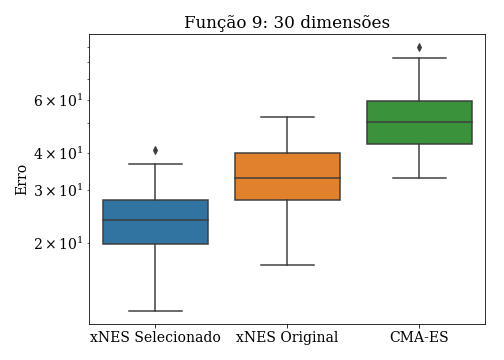
\includegraphics[width=2.0in]{figures/analysis_results/function=09_dim=30.png}
\label{fig:result_func09dim30}}
\hfil
\subfloat{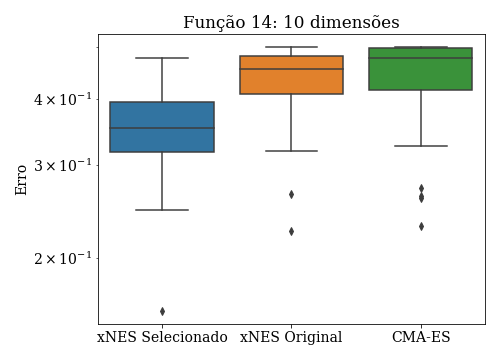
\includegraphics[width=2.0in]{figures/analysis_results/function=14_dim=10.png}
\label{fig:result_func14dim10}}
\subfloat{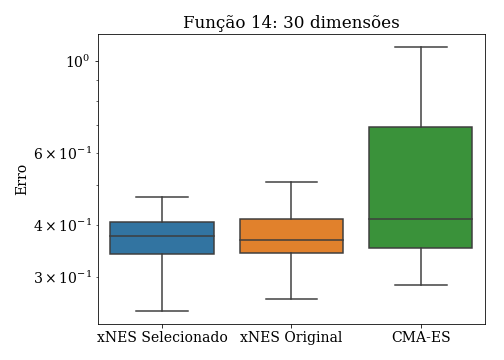
\includegraphics[width=2.0in]{figures/analysis_results/function=14_dim=30.png}
\label{fig:result_func14dim30}}
\caption{Comparação entre os algoritmos}
\label{fig:comp}
\end{figure*}
